%-------------------------------------------------------------------------
% td-info-S1-listes.tex
%-------------------------------------------------------------------------


\begin{td}[Distance de 2 points de l'espace]\label{td:distance}
\em
Définir la fonction {\tt distance} qui calcule la distance entre 2 points
$M_1$ et $M_2$ de l'espace, respectivement de coordonnées $(x_1,y_1,z_1)$ 
et $(x_2,y_2,z_2)$.
\end{td}

\begin{td}[Opérations sur les n-uplets]\label{td:n-uplet}\index[td]{opérations sur les n-uplets}
\em
Donner un exemple d'utilisation de chacune des opé\-ra\-tions  
sur les n-uplets décrites dans le tableau de la page \pageref{tab:sequences}.
\end{td}

\begin{td}[Pgcd et ppcm de 2 entiers (2)]\label{td:pgcdppcm}\index[td]{pgcd et ppcm de 2 entiers}
(voir TD \ref{td:pgcd})\\
\em
Définir une fonction qui calcule le pgcd et le ppcm de 2 entiers $a$ et $b$.
\end{td}

\begin{td}[Opérations sur les chaînes]\label{td:chaine}\index[td]{opérations sur les chaînes de caractères}
\em
Donner un exemple d'utilisation de chacune des opé\-ra\-tions  
sur les chaînes de caractères décrites dans le tableau de la page \pageref{tab:chaines}.
\end{td}

\begin{td}[Inverser une chaîne]\label{td:inverser}\index[td]{inverser une chaîne}
\em
Définir une fonction qui crée une copie d'une chaîne en inversant l'ordre des caractères.

\noindent\mbox{}\hspace*{1cm}\begin{py}{6cm}\tt
>>> inverser('inverser')\\
'resrevni'
\end{py}
\end{td}

\begin{td}[Caractères, mots, lignes d'une chaîne]\label{td:wc}\index[td]{caractères, mots, lignes d'une chaîne}
\em
Définir une fonction qui compte le nombre de caractères, le nombre de mots et le nombres de lignes
d'une chaîne de caractères.
\end{td}

\begin{td}[Opérations sur les listes (1)]\label{td:listes1}\index[td]{opérations sur les listes}
\em
Donner un exemple d'utilisation de chacune des opé\-ra\-tions  
sur les listes décrites dans le tableau de la page \pageref{tab:listes}.
\end{td}

\begin{td}[Opérations sur les listes (2)]\label{td:listes2}
\em
Vérifier que les opérations suivantes sont équivalentes deux à deux :
$$\begin{tabular}{l@{ et }l}
{\tt del s[i\char`:j]}	& {\tt s[i\char`:j] = []}\\
{\tt s.append(x)}	& {\tt s[len(s)\char`:len(s)] = [x]}\\
{\tt s.extend(x)}      	& {\tt s[len(s)\char`:len(s)]= x}\\
{\tt s.insert(i,x)}	& {\tt s[i\char`:i] = [x]}\\
{\tt s.remove(x)}	& {\tt del s[s.index(x)]}\\
{\tt s.pop(i)}		& {\tt x = s[i]; del s[i]}\\
\end{tabular}$$
\end{td}


\begin{td}[Sélection d'éléments]\label{td:collect}\index[td]{sélection d'éléments}
\em
\begin{enumerate}
\item Définir une fonction qui crée une liste {\tt t} composée des éléments d'une autre 
	liste {\tt s} qui vérifient une certaine condition {\tt p} ({\tt p(s[i]) == True}).
\item Définir une fonction qui supprime d'une liste {\tt s} les éléments qui ne vérifient
	pas une certaine condition {\tt p}.
\end{enumerate}
\end{td}

\begin{td}[Opérations sur les piles]\label{td:pile}\index[td]{opérations sur les piles}
\em
Définir les 4 opérations sur les piles définies ci-contre~: {\tt emptyStack}, {\tt topStack},
{\tt pushStack} et {\tt popStack}. On empilera et dépilera à la fin de la liste qui
sert à stocker les éléments de la pile.
\end{td}

\begin{td}[Opérations sur les files]\label{td:file}\index[td]{opérations sur les files}
\em
Définir les 4 opérations sur les files définies ci-contre~: {\tt emptyQueue}, {\tt topQueue},
{\tt pushQueue} et {\tt popQueue}. On enfilera en début de liste et on défilera à la fin de la liste qui
sert à stocker les éléments de la file.
\end{td}

\begin{td}[Produit de matrices]\label{td:matrices1}\index[td]{opérations sur les matrices}
\em
Définir la fonction qui calcule la matrice $C$, produit 
de 2 matrices $A$ et $B$ respectivement de dimensions $(n,r)$ et $(r,m)$.
$$c_{i,j} = \sum_{k=0}^{r-1}a_{ik}\cdot b_{kj}$$
\centerline{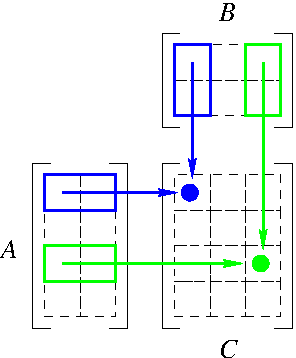
\includegraphics[width=4cm]{produit-matrices.pdf}}
\end{td}

\begin{td}[Annuaire téléphonique]\label{td:annuaire}\index[td]{annuaire téléphonique}
\em
On considère un annuaire téléphonique stocké sous la forme d'une liste de couples
{\tt (nom, téléphone)} (exemple : {\tt [('jean','0607080910'),('paul','0298000102')]}).
\begin{enumerate}
\item Définir une fonction qui retrouve dans un annuaire téléphonique
	le numéro de téléphone à partir du nom.
\item Définir la fonction inverse qui retrouve 
	le nom à partir du numéro de téléphone.
\end{enumerate}
\end{td}

\begin{td}[Recherche dichotomique]\label{td:dicho}\index[td]{recherche dichotomique}
\em
La recherche dichotomique présentée ci-contre n'assure pas de trouver la première occurence
d'un élément {\tt x} dans une liste {\tt t} triée.\\
Modifier l'algorithme de recherche dichotomique proposé pour rechercher la
première occurence d'un élément {\tt x} dans une liste {\tt t} triée.
\end{td}

\begin{td}[Liste ordonnée]\label{td:enordre}\index[td]{liste ordonnée}
\em
Définir une version itérative de la fonction récursive {\tt enOrdre}
définie ci-dessous. On appliquera la méthode de transformation décrite en
section \ref{methode:recursivite} page \pageref{methode:recursivite}.

\footnotesize
\begin{verbatim}
def enOrdre(t,debut,fin):
    assert type(t) is list
    assert 0 <= debut <= fin < len(t)
    ok = False
    if debut == fin: ok = True
    else:
        if t[debut] <= t[debut+1]: 
            ok = enOrdre(t,debut+1,fin)
    return ok
\end{verbatim}

\end{td}

\begin{td}[Tri d'un annuaire téléphonique]\label{td:tri1}\index[td]{tri d'un annuaire}
\em
On considère un annuaire téléphonique stocké sous la forme d'une liste de couples
{\tt (nom, téléphone)} (exemple : {\tt [('paul','0607080910'),('jean','0298000102')]}).

Définir une fonction qui trie un annuaire téléphonique par ordre alphabétique des noms.
\end{td}

\begin{td}[Complexité du tri par sélection]\label{td:tri2}\index[td]{complexité du tri par sélection}
\em
Montrer que la complexité du tri par sélection est :
\begin{enumerate}
\item en $O(n)$ en ce qui concerne les échanges de valeurs au sein d'une liste
	de longueur $n$,
\item en $O(n^2)$ en ce qui concerne les comparaisons entre éléments de la liste.
\end{enumerate}
\end{td}

\begin{td}[Tri par insertion]\label{td:tri3}\index[td]{tri par insertion}
\em
Exécuter à la main l'appel {\tt triInsertion([9,8,7,6,5,4],1,4)} en donnant
les valeurs des variables {\tt i}, {\tt k}, {\tt x} et {\tt t} à la fin de chaque
itération de la boucle {\tt while} (lignes 7--9 de la version itérative de 
l'algorithme).

\begin{lstlisting}[title={\bf Tri par insertion}]
def triInsertion(t,debut,fin):
    assert type(t) is list
    assert 0 <= debut <= fin < len(t)
    for k in range(debut+1,fin+1):
        i = k - 1
        x = t[k]
        while i >= debut and t[i] > x:
            t[i+1] = t[i]
            i = i - 1
        t[i+1] = x
    return
\end{lstlisting}

\end{td}

\begin{td}[Comparaison d'algorithmes (1)]\label{td:exectri1}\index[td]{comparaison d'algorithmes de tri}
\em
Comparer les temps d'exécution des versions récursive et itérative du tri rapide pour
différentes tailles de liste.

On pourra utiliser la fonction {\tt random()} ou {\tt randint(min,max)} du module standard
{\tt random} pour générer des listes de nombres aléatoires, et la fonction {\tt time()}
du module standard {\tt time} pour mesurer le temps avant et après l'appel des
fonctions.
\end{td}

\begin{td}[QCM (4)]\label{td:qcmListes}(un seul item correct par question)
\index[td]{contrôle d'attention}
\em
\begin{enumerate}
\item Le type d'une variable définit 
	\begin{enumerate}
	\item l'ensemble des noms qu'elle peut prendre.
	\item le regroupement fini des données qui la composent et
		dont le nombre n'est pas fixé {\em a priori}.
	\item l'ensemble des valeurs qu'elle peut prendre et 
		l'ensemble des opérations qu'elle peut subir.
	\item le regroupement hiérarchique des données qui la composent 
	\end{enumerate}

\item Une séquence est 
	\begin{enumerate}
	\item un regroupement fini de données dont le nombre 
		n'est pas fixé {\em a priori}.
	\item une collection d'éléments, appelés « sommets », et de 
		relations entre ces sommets.
	\item une collection non ordonnée d'éléments.
	\item une suite ordonnée d'éléments
		accessibles par leur rang dans la séquence.
	\end{enumerate}

\item Parmi les exemples suivants, le seul exemple de séquence est
	\begin{enumerate}
	\item le tableau final d'un tournoi de tennis.
	\item la carte routière.
	\item la classification des espèces animales.
	\item la main au poker.
	\end{enumerate}

\item Parmi les types suivants, un seul n'est pas une variante de séquence. Lequel ?
	\begin{enumerate}
	\item le n-uplet.
	\item la chaîne de caractères.
	\item le dictionnaire.
	\item la pile.
	\end{enumerate}

\item Dans une liste 
	\begin{enumerate}
	\item tous les éléments sont du même type.
	\item les éléments peuvent avoir des types différents.
	\item les éléments ne peuvent pas être des dictionnaires.
	\item les éléments ont comme type un des types de base ({\tt bool},{\tt int},{\tt float}).
	\end{enumerate}

\item Dans la liste multidimensionnelle {\tt s = [[1,2,3,4],[5,6,7],[8,9]]} que vaut {\tt s[1][1]} ?
	\begin{enumerate}
	\item 1.
	\item 2.
	\item 5.
	\item 6.
	\end{enumerate}

\item Une pile est une séquence dans laquelle 
	\begin{enumerate}
	\item on ne peut ajouter un élément qu'à une seule extrémité 
		et ne supprimer un élément qu'à l'autre extrémité.
	\item on ne peut ajouter un élément qu'à une seule extrémité
		et en supprimer n'importe où.
	\item on ne peut ajouter et supprimer un élément
		qu'à une seule extrémité.
	\item on ne peut supprimer un élément qu'à une seule extrémité
		et en ajouter n'importe où.
	\end{enumerate}

\item Une file est une séquence dans laquelle 
	\begin{enumerate}
	\item on ne peut ajouter un élément qu'à une seule extrémité 
		et ne supprimer un élément qu'à l'autre extrémité.
	\item on ne peut ajouter un élément qu'à une seule extrémité
		et en supprimer n'importe où.
	\item on ne peut ajouter et supprimer un élément
		qu'à une seule extrémité.
	\item on ne peut supprimer un élément qu'à une seule extrémité
		et en ajouter n'importe où.
	\end{enumerate}

\item La recherche séquentielle d'un élément dans une liste consiste à 
	\begin{enumerate}
	\item rechercher le minimum de la liste et à le mettre en début de liste 
		en l'échangeant avec cet élément.
	\item rechercher le maximum de la liste et à le mettre en début de liste 
		en l'échangeant avec cet élément.
	\item comparer l'élément recherché successivement à tous les 
		éléments de la liste jusqu'à trouver une correspondance.
	\item comparer l'élément recherché avec l'élément milieu de la liste
		et poursuivre de même dans la sous-liste de droite ou 
		dans la sous-liste de gauche à l'élément milieu.
	\end{enumerate}

\item Dans le tri par insertion 
	\begin{enumerate}
	\item on partage la liste à trier en deux sous-listes telles que tous les éléments 
		de la première soient inférieurs à tous les éléments de la seconde,
		puis on trie les deux sous-listes selon le même processus jusqu'à 
		avoir des sous-listes réduites à un seul élément.
	\item on trie successivement les premiers éléments de la liste : à la $i^{\grave eme}$ étape, 
		on place le $i^{\grave eme}$ élément à son rang 
		parmi les $i-1$ éléments précédents qui sont déjà triés entre eux.
	\item on parcourt la liste en commençant par la fin, en effectuant un échange à
		chaque fois que l'on trouve deux éléments successifs qui ne sont pas 
		dans le bon ordre.
	\item on recherche le minimum de la liste à trier, on le met en début de liste 
		en l'échangeant avec le premier élément et on recommence sur le reste de la liste.
	\end{enumerate}

\end{enumerate}
\end{td}

\begin{td}[Génération de séquences]\label{td:alea}
\index[td]{génération de séquences}
\em
A l'aide de la fonction {\tt randint(min,max)} du module standard {\tt random},
Définir les fonctions de génération suivantes :
\begin{enumerate}
\item {\tt liste(n)} : génère une liste de {\tt n} entiers compris entre {\tt 0} et {\tt n}.
\item {\tt nuplet(n)} : génère un n-uplet de {\tt n} entiers compris entre {\tt 0} et {\tt n}.
\item {\tt chaine(n)} : génère une chaîne de {\tt n} caractères imprimables.
\end{enumerate}
\end{td}

\begin{td}[Application d'une fonction à tous les éléments d'une liste]\label{td:foreach}
\index[td]{application d'une fonction}
\em
Définir une fonction qui applique la même fonction {\tt f} à tous les éléments d'une liste {\tt s}.

Exemples : 
\begin{tabular}[t]{l@{ , }l@{ $\rightarrow$ }l}
{\tt s = [-1,2,3,-4]}		& {\tt f = abs} & {\tt s = [1,2,3,4]}\\
{\tt s = [pi/2,pi,3*pi/2]}	& {\tt f = sin} & {\tt s = [1,0,-1]}
\end{tabular}
\end{td}


\begin{td}[Que fait cette procédure ?]\label{td:trishell}
\index[td]{que fait cette procédure ?}
\em
On considère la procédure {\tt f} ci-dessous.

\noindent\mbox{}\hspace*{1cm}\begin{py}{7cm}\tt
\begin{verbatim}
def f(t,debut,fin):
    m = (debut + fin)/2
    while m > 0:
        for i in range(m,fin+1):
            j = i - m
            while j >= debut:
                print(m,i,j,t)
                if t[j] > t[j+m]:
                    t[j],t[j+m] = t[j+m],t[j]
                    j = j - m
                else: j = debut-1
        m = m/2
    return 
\end{verbatim}
\end{py}

\vspace*{2mm}

\begin{enumerate}
\item Tracer l'exécution {\em à la main} de l'appel {\tt f([4,2,1,2,3,5],0,5)}.
\item Que fait cette procédure ?
\end{enumerate}

\end{td}


\begin{td}[Codes ASCII et chaînes de caractères]\label{td:asciichaines}\index[td]{codes ASCII et chaînes de caractères}
\em
\begin{enumerate}
\item Ecrire un algorithme qui fournit le tableau des codes ASCII
        (annexe \ref{ascii} page \pageref{ascii}) associé
        à une chaîne (exemple : {\tt 'bon'} $\rightarrow$ {\tt [98, 111, 110]}).
\item Ecrire un algorithme qui donne la chaîne de caractères associée à un tableau de codes
        ASCII (exemple : {\tt [98, 111, 110]} $\rightarrow$ {\tt 'bon'}).
\end{enumerate}
\end{td}

\begin{td}[Opérations sur les matrices]\label{td:matrices2}\index[td]{opérations sur les matrices}
\em
\begin{enumerate}
\item Définir une fonction qui teste si une liste {\tt m} est une matrice.
\item Définir une fonction qui teste si une matrice {\tt m} est une matrice carrée.
\item Définir une fonction qui teste si une matrice {\tt m} est une matrice symétrique.
\item Définir une fonction qui teste si une matrice {\tt m} est une matrice diagonale.
\item Définir une fonction qui multiplie une matrice {\tt m} par un scalaire {\tt x}.
\item Définir une fonction qui détermine la transposée d'une matrice {\tt m}.
\end{enumerate}
\end{td}


\begin{td}[Recherche d'un motif]\label{td:motif}\index{recherche dans une séquence!recherche d'un motif}
\index[td]{recherche d'un motif}
\em
Définir un algorithme qui recherche la première occurence d'une séquence {\tt m}
au sein d'une autre séquence {\tt t}.
\end{td}

\begin{td}[Recherche de toutes les occurences]\label{td:occurs}
\index[td]{recherche de toutes les occurences}
\em
Définir une fonction qui retourne la liste des rangs de toutes les occurences
d'un élément {\tt x} dans une liste {\tt t}.
\end{td}

\begin{td}[Tri bulles]\label{td:bulles}\index{tri d'une séquence!tri bulles}
\index[td]{tri bulles}
\em
Dans le tri bulles, on parcourt la liste en commençant par la fin, en effectuant un échange à
chaque fois que l'on trouve deux éléments successifs qui ne sont pas dans le bon ordre.

\noindent Définir une fonction qui trie une liste selon la méthode du tri bulles.
\end{td}

\begin{td}[Méthode d'élimination de {\sc Gauss}]\label{td:gauss}\index[td]{méthode d'élimination de {{\sc Gauss}}}
\em
L'objectif est ici de 
résoudre dans $\mathbb{R}$ un système de $n$ équations linéaires
à $n$ inconnues, homogènes ou non homogènes, du type $A\cdot x = b$ :
$$\left\{
\begin{array}{r@{\ +\ }r@{\ +\ }r@{\ +\ }r@{\ =\ }r}
a_{00}x_0     & a_{01}x_1     & \cdots & a_{0(n-1)}x_{(n-1)}     & b_0      \\
a_{10}x_0     & a_{11}x_1     & \cdots & a_{1(n-1)}x_{(n-1)}     & b_1      \\
\cdots        & \cdots        & \cdots & \cdots                  & \cdots   \\
a_{(n-1)0}x_0 & a_{(n-1)1}x_1 & \cdots & a_{(n-1)(n-1)}x_{(n-1)} & b_{(n-1)}
\end{array}
\right.$$
Définir une fonction {\tt solve(a,b)} qui retourne le vecteur {\tt x}
solution du système linéaire $A\cdot x = b$ selon la méthode d'élimination de 
{\sc Gauss} décrite en section \ref{gauss} page \pageref{gauss}.
\end{td}


\begin{td}[Comparaison d'algorithmes de recherche.]\label{td:exectri2}\index[td]{comparaison d'algorithmes de recherche}
\em
Comparer les temps d'exécution des versions récursive et itérative des
2 méthodes de recherche développées dans le cours (recherche séquentielle, recherche dichotomique).

On pourra utiliser la fonction {\tt random()} ou {\tt randint(min,max)} du module standard
{\tt random} pour générer des listes de nombres aléatoires, et la fonction {\tt time()}
du module standard {\tt time} pour mesurer le temps avant et après l'appel des
fonctions.
\end{td}

\begin{td}[Comparaison d'algorithmes de tri]\label{td:exectri3}\index[td]{comparaison d'algorithmes de tri}
\em
Comparer les temps d'exécution des différentes versions récursives et itératives des
3 méthodes de tri développées dans le cours (tri par sélection, tri par insertion, tri rapide).

On pourra utiliser la fonction {\tt random()} ou {\tt randint(min,max)} du module standard
{\tt random} pour générer des listes de nombres aléatoires, et la fonction {\tt time()}
du module standard {\tt time} pour mesurer le temps avant et après l'appel des
fonctions.
\end{td}
